\begin{figure*}[t]
\centering
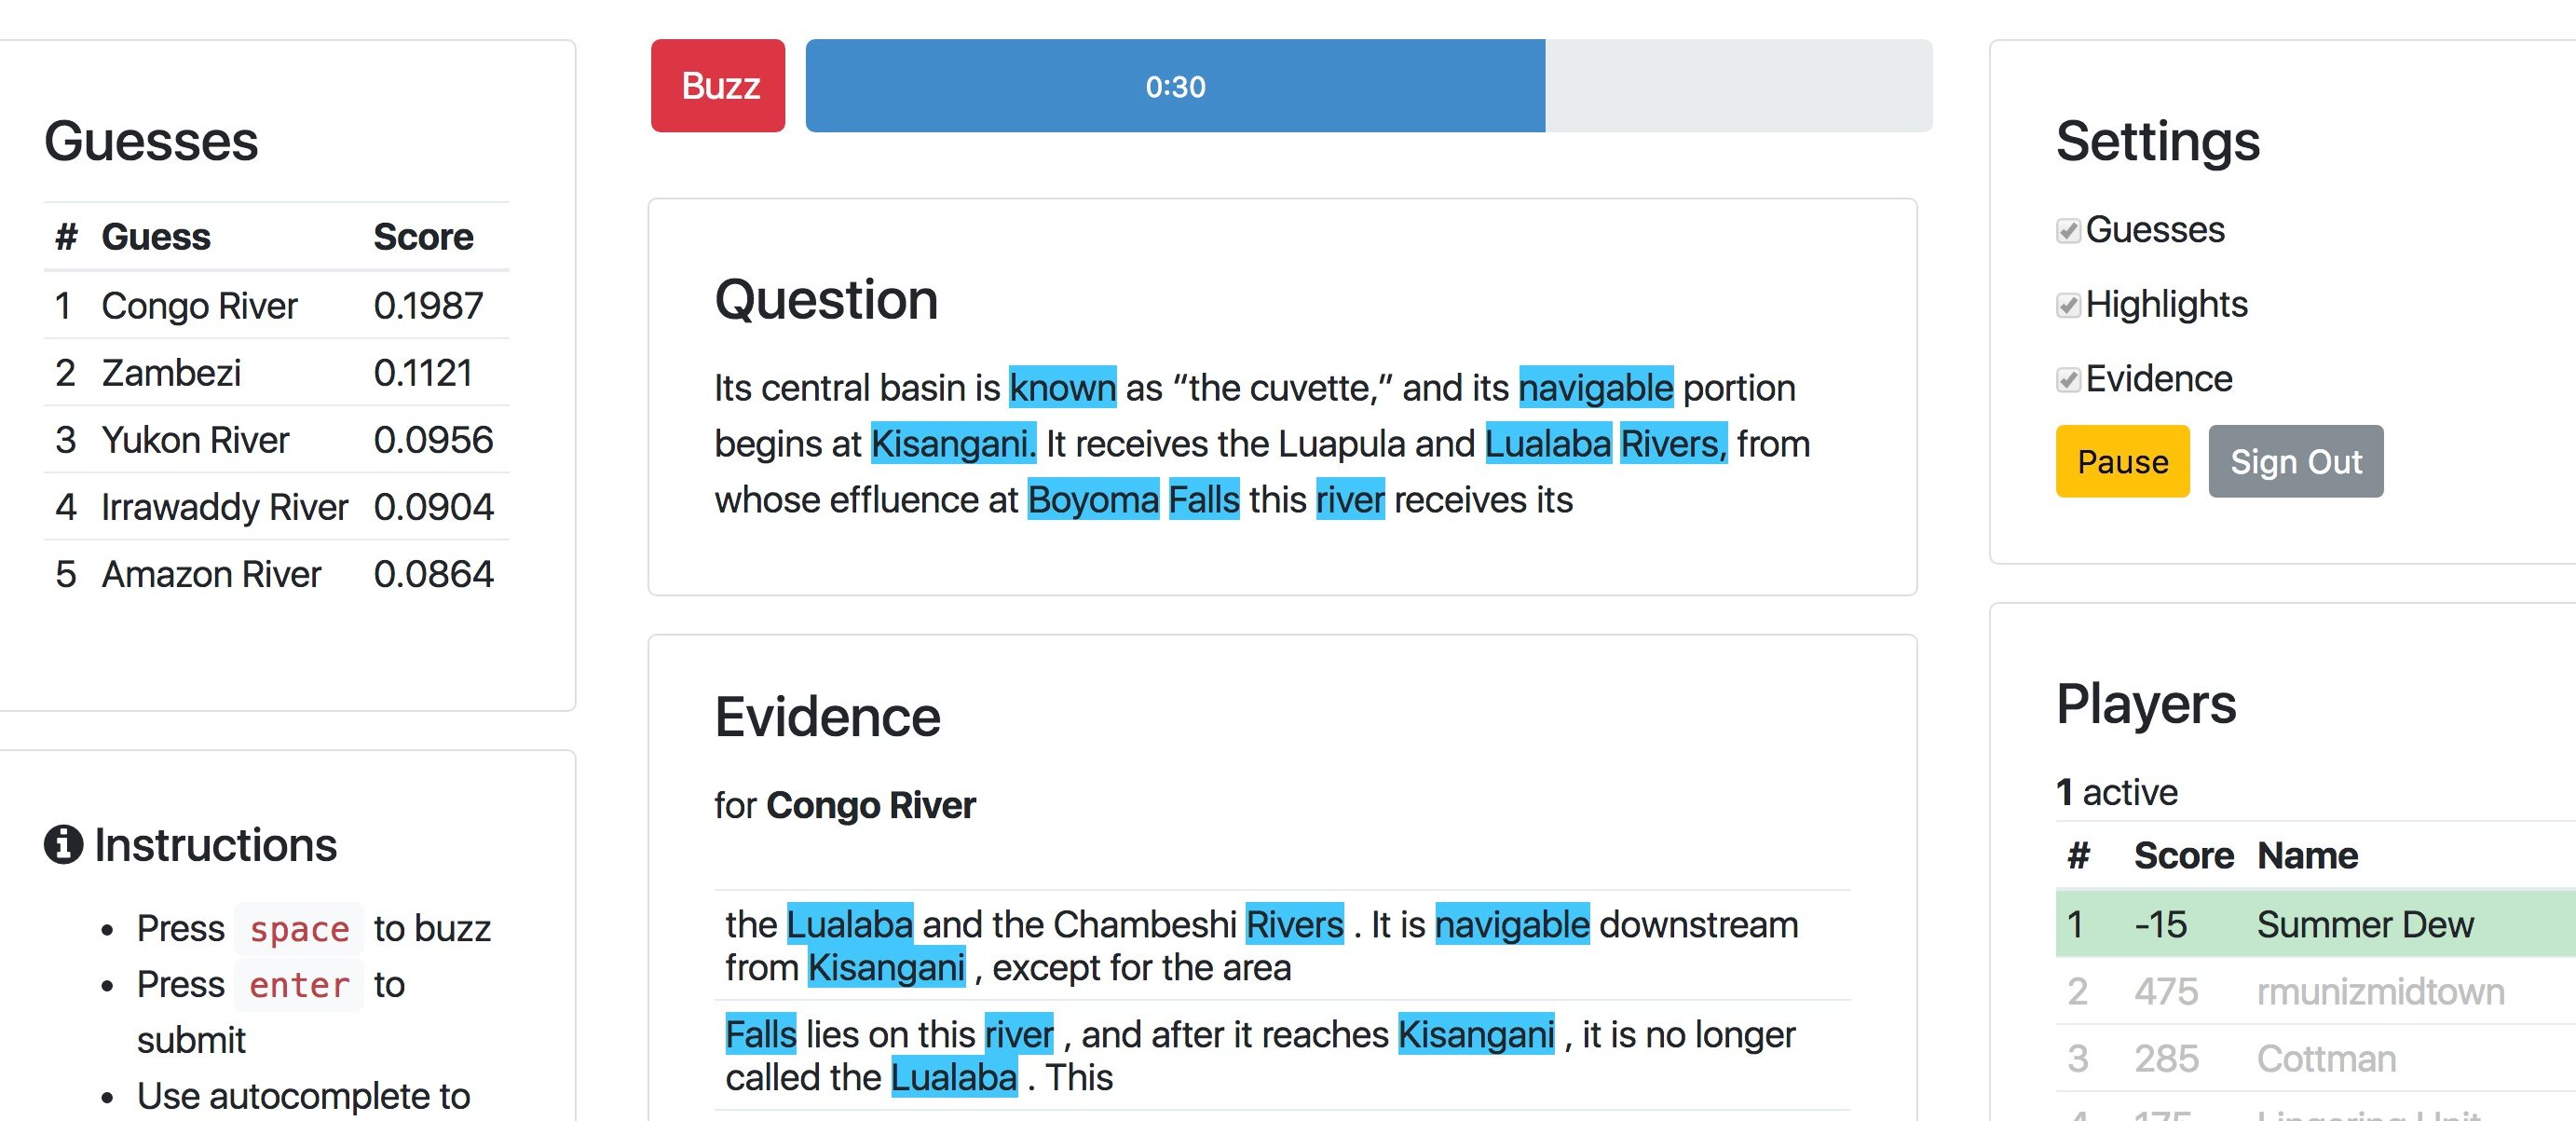
\includegraphics[width=0.85\textwidth]{screenshot_all}
\caption{\label{fig:screenshot} Screenshot of the interface. Question is
    displayed in the middle area word-by-word, with question highlights
    displayed in the same panel. Guesses are listed in the panel on the left.
    Evidence is in the panel below.}
\end{figure*}

\section{Interface Design}
\label{sec:design}

% 1. lead-in
We design our \qb{} interface (Figure~\ref{fig:screenshot}) to
\emph{visualize} the three interpretations described in the previous
section. This section introduces the visualizations, placement, and
interactivity of the interface. 

% 2. design principle
To make \qb{} players feel at home, we follow the general framework
of~\url{Protobowl.com}, a popular \qb{} platform
% inspired by Boyd-Graber~\etal{}~\cite{boydgraber2012besting} 
that many
players actively use for practice.  The \textbf{Question} area is
in the center, and the question is displayed word-by-word in
the text box. A \textbf{Buzz} button is located close above the
question area, and to further reduce the distraction from the question
area, players can also buzz in using the space key. After buzzing, the
player have eight seconds to enter and select an answer from
a drop-down menu.

\begin{figure}[H]
\centering
\fbox{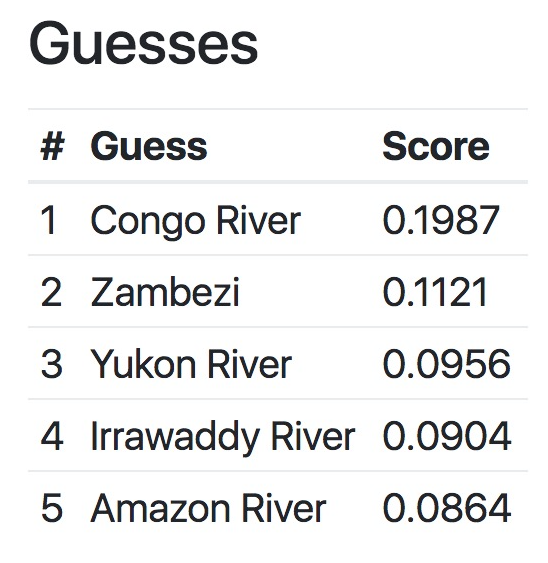
\includegraphics[width=0.4\columnwidth]{screenshot_guesses}}
\end{figure}

% 3. guesses
\textbf{Guesses} show the answers the computer is considering along
with the associated score.  Top ten answers are sorted according to
their score (the system prefers higher scores).  This helps convey
when the model is uncertain (e.g., if all of the guesses have a low
score).

\begin{figure}[H]
\centering
\fbox{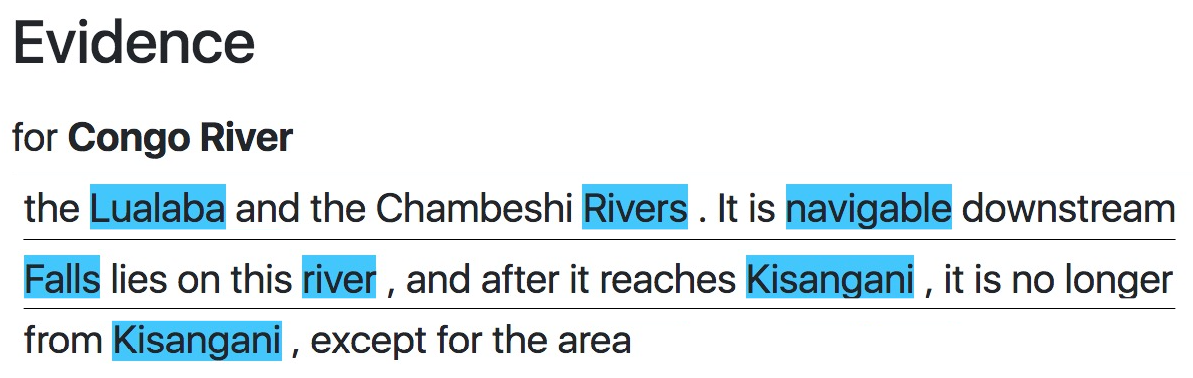
\includegraphics[width=0.85\columnwidth]{screenshot_evidence}}
\end{figure}

% 4. evidence
To inform the player of how the model's prediction is supported by
training examples, \textbf{Evidence} shows the relevant snippets of
the most salient training examples for the top guess. It is located
below the question area and has the same width to provide a direct
comparison against the input question. Each line of the text area
shows the snippet of one selected document.

\begin{figure}[H]
\centering
\fbox{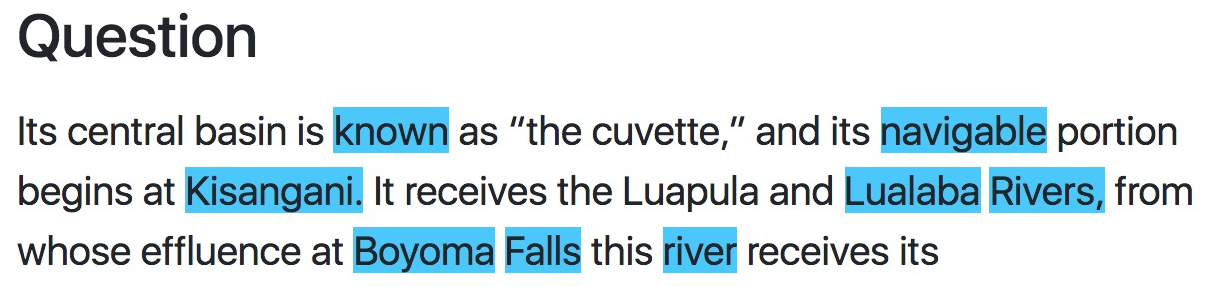
\includegraphics[width=0.85\columnwidth]{screenshot_highlight}}
\end{figure}

% 5. highlight
We use \textbf{Highlight} to visualize the most salient words in both
the input question and the evidence snippets. These words are selected
for the top guess. As introduced in the previous section, we first
highlight important words in the training example snippets using an
\abr{api} of \abr{es}, then find their appearances in the input and
highlight those too. 

% \jbgcomment{This is very unclear.  Rewrite, use concrete words
% (instead of ``visualize''.  Give example, and use ``evidence
% highlight'' and ``question highlight'' if you're going to have two
% terms.}

% 6. combinations, need to expand
Multiple interpretations can be shown in combination. The
combination of highlight and evidence has a compounding effect: when
both are enabled, players see highlighted words in both the question
and the evidence (for example in Figure~\ref{fig:screenshot});
when highlight is enabled without evidence, players only see
highlights in the question.

% \jbgcomment{The below paragraph makes it seem like we're trying to
%   make highlights win.  Say that it needs to be the same width as
%   question, so we place it below.  Then say that we discuss this
%   choice in the limitations section at the end of the paper.}

% 7. hint on UI future work
Our design goal is to minimize distraction from the
question area while boosting the competitiveness of the player. So we place
the question area in the middle and have all interpretations around it.
% This might give highlight visualization an unfair amount of
% attention, since it is in a more central position.
It is difficult to ensure that different forms of
interpretations are exposed to the users equally, as some forms (e.g.,
evidence) are inherently less intuitive to visualize. However,
all interpretations must be implemented in an interface for a
real-world evaluation; we discuss the limitations of our design and
future work in Section~\ref{sec:discussion}.
